%!TEX root = ../Thesis.tex
%!TEX program = xelatex
\documentclass[../Thesis]{subfiles}

% 本文
\begin{document}
\chapter{実験}
\section{実験環境}
本研究における実験環境を\tref{tab01}に示す。

\begin{table}[h]
  \centering
	\caption{使用データ}
	\label{tab01}
	\begin{tabular}{l l}
		\hline
		CPU & Intel® Core™ i7-7500U @ 2.70GHz 2.90GHz\\
		メモリ & 8.00 GB \\
		OS & Windows 10 Pro \\
		開発環境 & Microsoft Visual Studio Code 1.52.0 \\
		使用言語 & Python 3.8.0 \\
		使用ライブラリ & OpenCV 4.2.0 \\ \hline
	\end{tabular}
\end{table}

\section{使用データ}
本研究では平成29年7月九州北部豪雨のドローン空撮映像\cite{web02}を用いた.空撮映像の詳細を\tref{tab02}と\tref{tab03}に示す.

\begin{table}[h]
	\centering
	\caption{使用データ}
	\label{tab02}
	\begin{tabular}{l l}
		\hline
		災害名称 & 平成29年7月九州北部豪雨 \\
		撮影箇所 & 福岡県朝倉市赤谷川 \\
		撮影日時 & 平成29年7月7日15時30分 \\
		解像度 & 1920 × 1080 pixel\\
		提供 & 国土地理院 \\ \hline
	\end{tabular}
\end{table}

\begin{table}[h]
	\centering
	\caption{使用データ}
	\label{tab03}
	\begin{tabular}{l l}
		\hline
		災害名称 & 平成29年7月九州北部豪雨 \\
		撮影箇所 & 福岡県 \\
		撮影日時 & 平成29年7月7日x時x分 \\
		解像度 & 1920 × 1080 pixel\\
		提供 & 国土地理院 \\ \hline
	\end{tabular}
\end{table}


\section{実験結果}
\subsection{入力画像}
実験に使用したドローン空撮映像から切り取ったフレーム画像を\fref{img01}と\fref{img02}に示す。

\begin{figure}[h]
	\centering
	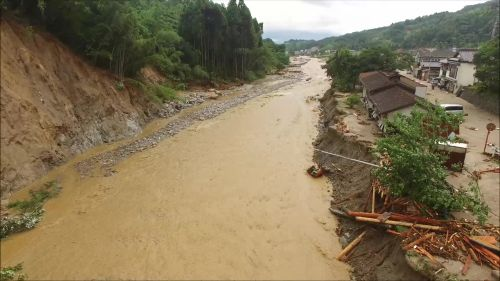
\includegraphics[width=8cm]{img/original1.png}
	\caption{入力画像(実験Ⅰ)}
	\label{img01}
\end{figure}

\begin{figure}[h]
	\centering
	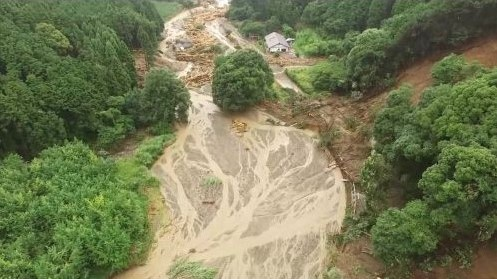
\includegraphics[width=8cm]{img/original2.png}
	\caption{入力画像(実験Ⅱ)}
	\label{img02}
\end{figure}


\subsection{領域分割}
前節の入力画像をMean-Shift法にて領域分割した結果を\fref{img03}と\fref{img04}に示す。

\begin{figure}[h]
	\centering
	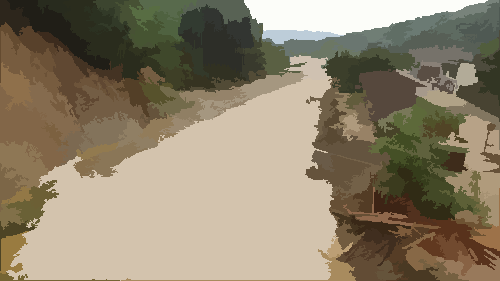
\includegraphics[width=8cm]{img/meanshift1.png}
	\caption{領域分割結果(実験Ⅰ)}
	\label{img03}
\end{figure}
\begin{figure}[h]
	\centering
	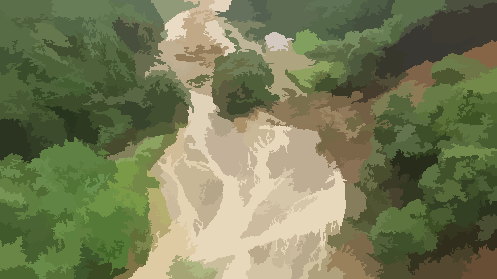
\includegraphics[width=8cm]{img/meanshift2.png}
	\caption{領域分割結果(実験Ⅱ)}
	\label{img04}
\end{figure}


\subsection{ヒストグラム均一化}
領域分割を適用した画像にCLAHEのアルゴリズムにてヒストグラム均一化を行った結果を\fref{img05}と\fref{img06}に示す。

\begin{figure}[h]
	\centering
	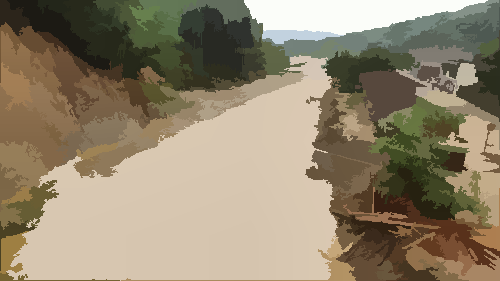
\includegraphics[width=8cm]{img/equalization1.png}
	\caption{ヒストグラム均一化結果(実験Ⅰ)}
	\label{img05}
\end{figure}
\begin{figure}[h]
	\centering
	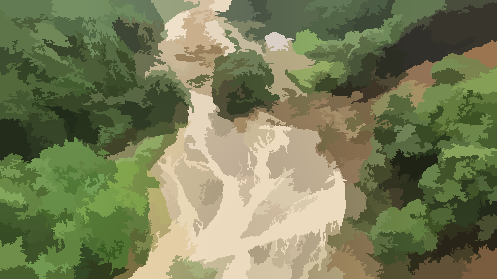
\includegraphics[width=8cm]{img/equalization2.png}
	\caption{ヒストグラム均一化結果(実験Ⅱ)}
	\label{img06}
\end{figure}

\subsection{災害領域検出}
\label{detection}
ヒストグラム均一化を適用した画像に対し閾値処理にて災害領域である斜面崩壊・浸水領域を検出した結果を\fref{img07}--\fref{img10}に示す。

\begin{figure}[h]
	\centering
	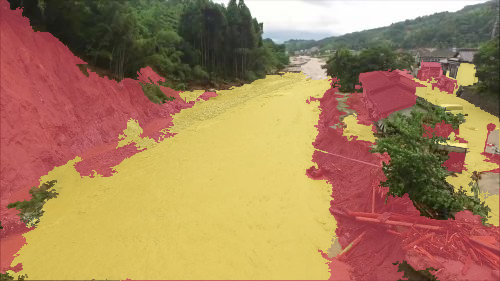
\includegraphics[width=8cm]{img/detection1.png}
	\caption{災害領域検出(実験Ⅰ)}
	% \caption{斜面崩壊領域検出(実験Ⅰ)}
	\label{img07}
\end{figure}
\begin{figure}[h]
	\centering
	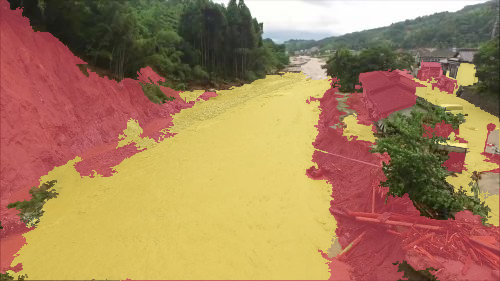
\includegraphics[width=8cm]{img/detection1.png}
	\caption{災害領域検出(実験Ⅱ)}
	\label{img08}
\end{figure}

% \begin{figure}[h]
% 	\centering
% 	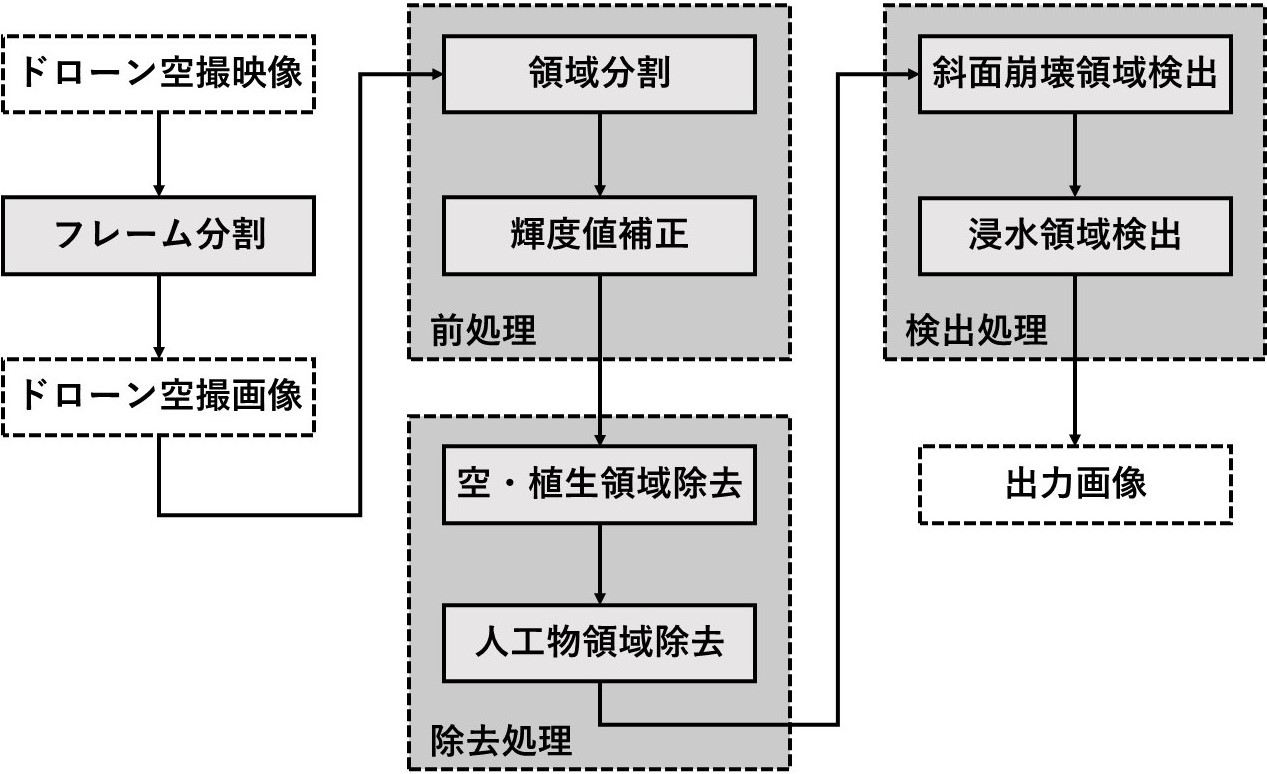
\includegraphics[width=8cm]{img/howto3.jpg}
% 	\caption{浸水領域検出(実験Ⅰ)}
% 	\label{img09}
% \end{figure}
% \begin{figure}[h]
% 	\centering
% 	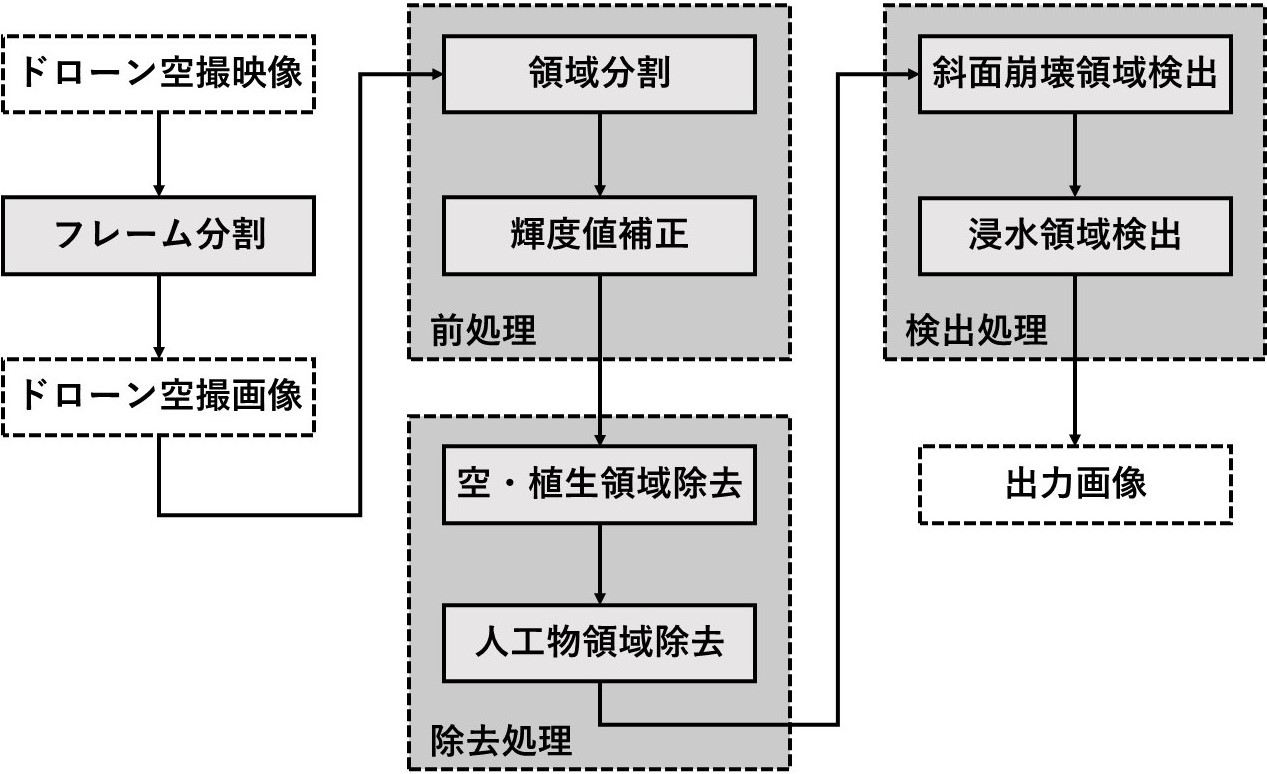
\includegraphics[width=8cm]{img/howto3.jpg}
% 	\caption{浸水領域検出(実験Ⅱ)}
% 	\label{img10}
% \end{figure}

\subsection{不要領域除去}
\label{rejection}
ヒストグラム均一化を適用した画像に対し閾値処理にて不要領域である植生・空・瓦礫・建物領域を検出した結果を\fref{img11}--\fref{img18}に示す。


\begin{figure}[h]
	\centering
	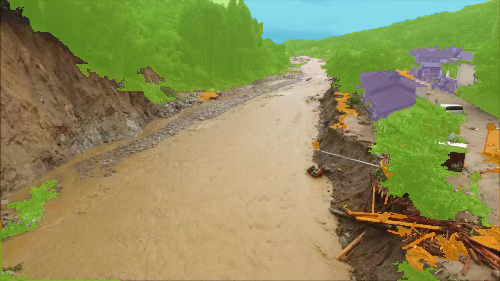
\includegraphics[width=8cm]{img/rejection1.png}
	\caption{不要領域検出(実験Ⅰ)}
	% \caption{植生領域検出(実験Ⅰ)}
	\label{img11}
\end{figure}
\begin{figure}[h]
	\centering
	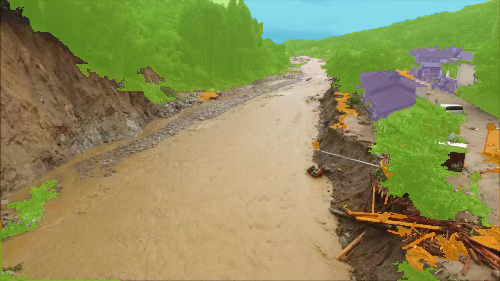
\includegraphics[width=8cm]{img/rejection1.png}
	\caption{不要領域検出(実験Ⅱ)}
	% \caption{植生領域検出(実験Ⅱ)}
	\label{img12}
\end{figure}

% \begin{figure}[h]
% 	\centering
% 	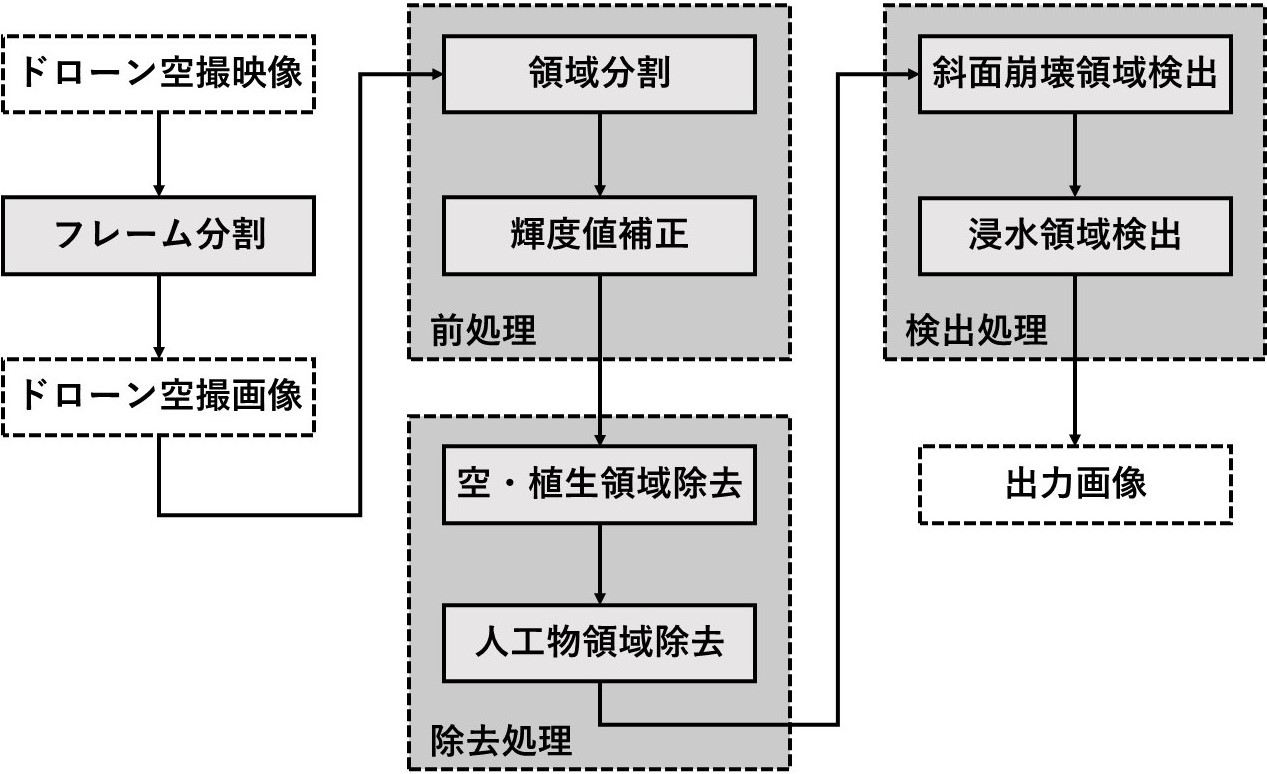
\includegraphics[width=8cm]{img/howto3.jpg}
% 	\caption{空領域検出(実験Ⅰ)}
% 	\label{img13}
% \end{figure}
% \begin{figure}[h]
% 	\centering
% 	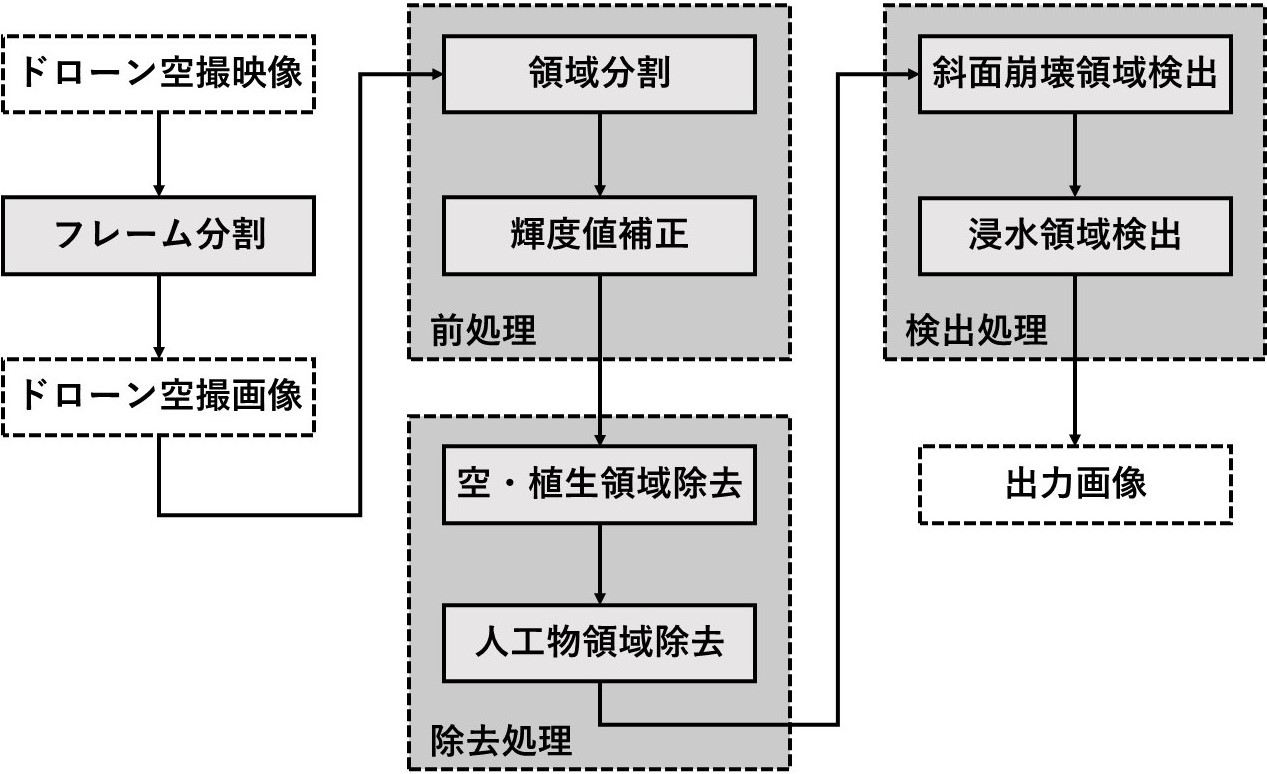
\includegraphics[width=8cm]{img/howto3.jpg}
% 	\caption{空領域検出(実験Ⅱ)}
% 	\label{img14}
% \end{figure}


% \begin{figure}[h]
% 	\centering
% 	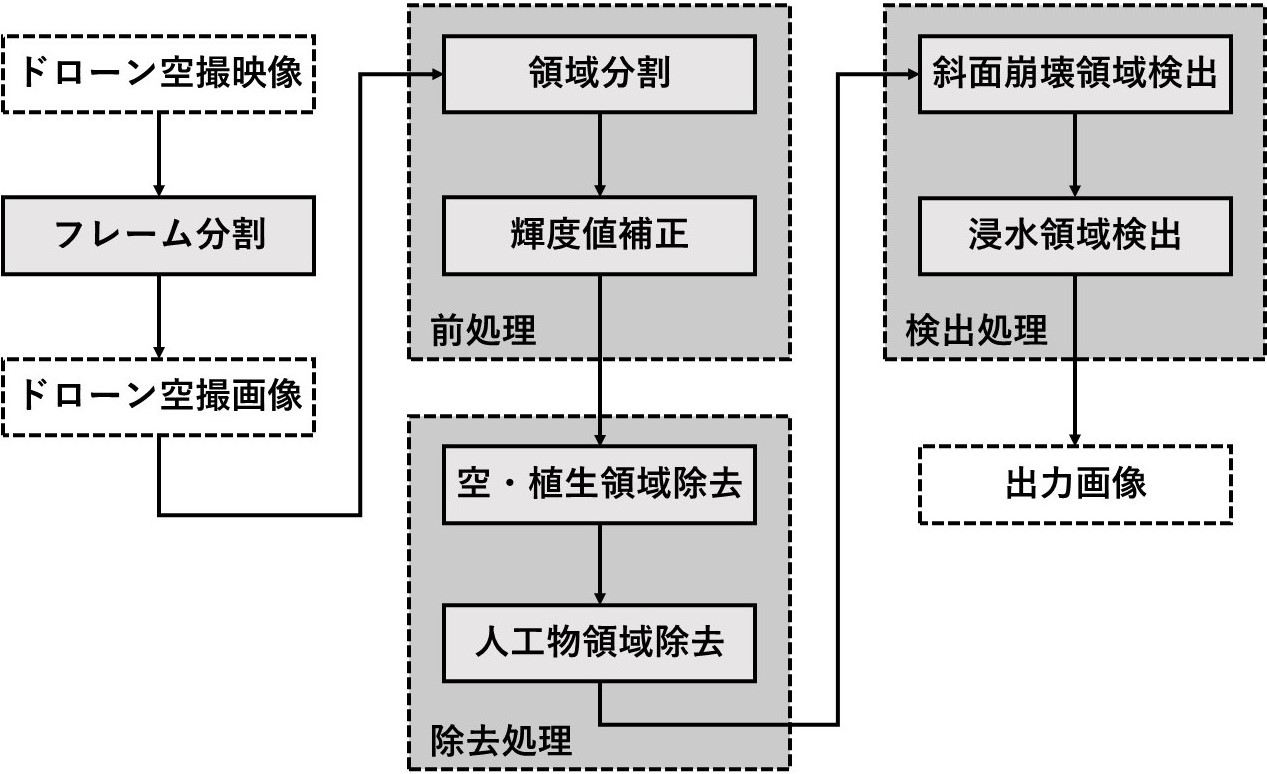
\includegraphics[width=8cm]{img/howto3.jpg}
% 	\caption{瓦礫領域検出(実験Ⅰ)}
% 	\label{img15}
% \end{figure}
% \begin{figure}[h]
% 	\centering
% 	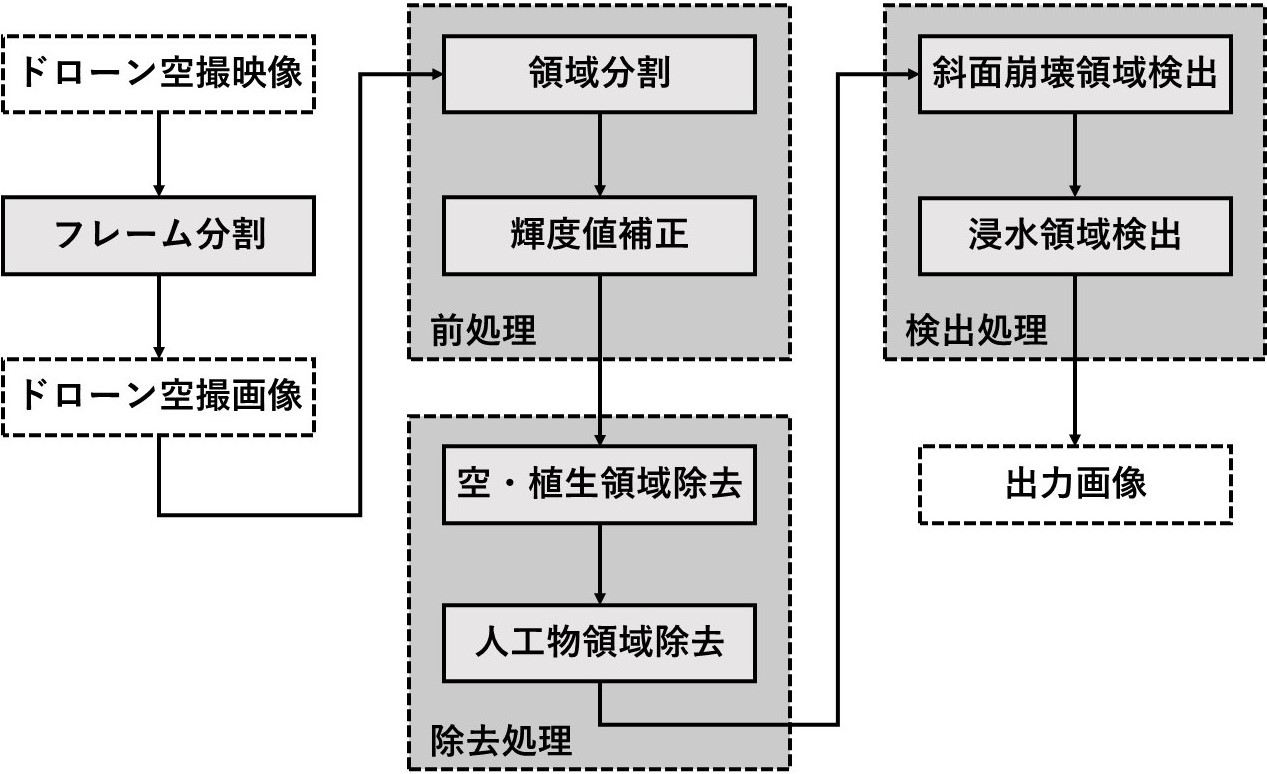
\includegraphics[width=8cm]{img/howto3.jpg}
% 	\caption{瓦礫領域検出(実験Ⅱ)}
% 	\label{img16}
% \end{figure}

% \begin{figure}[h]
% 	\centering
% 	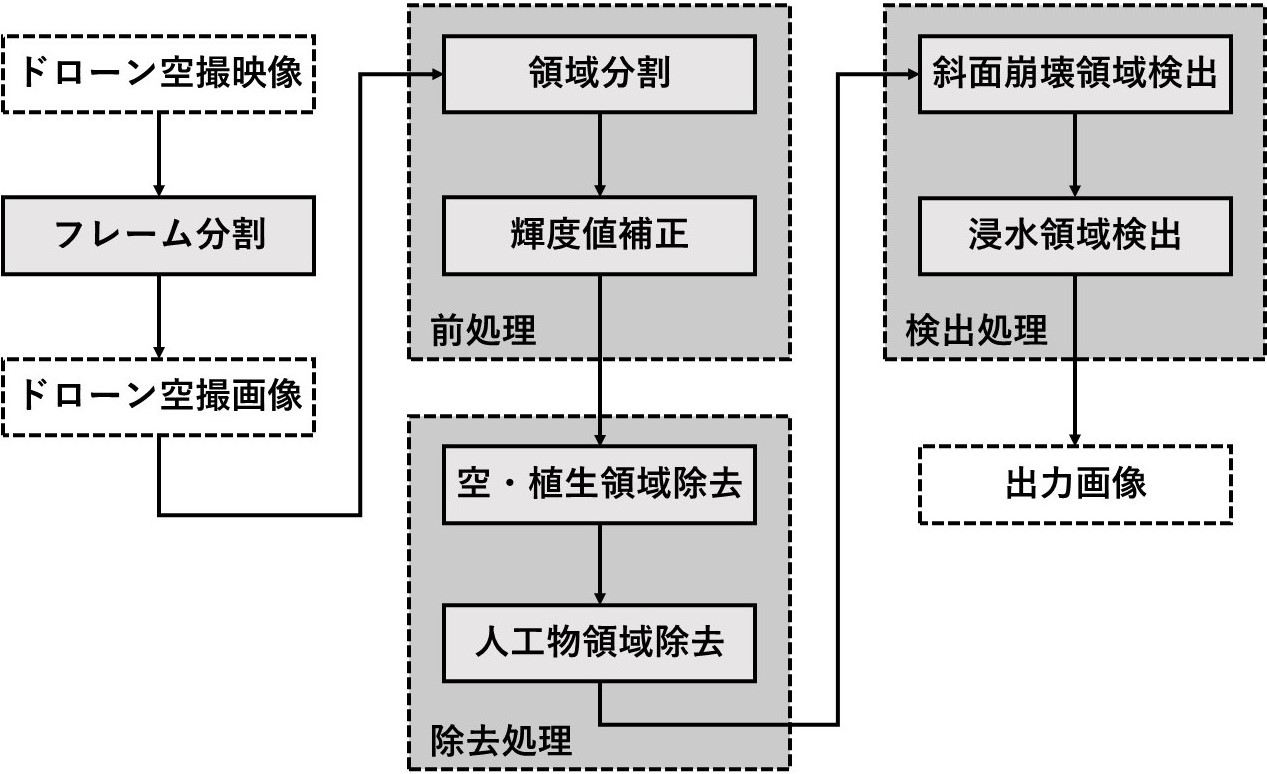
\includegraphics[width=8cm]{img/howto3.jpg}
% 	\caption{建物領域検出(実験Ⅰ)}
% 	\label{img17}
% \end{figure}
% \begin{figure}[h]
% 	\centering
% 	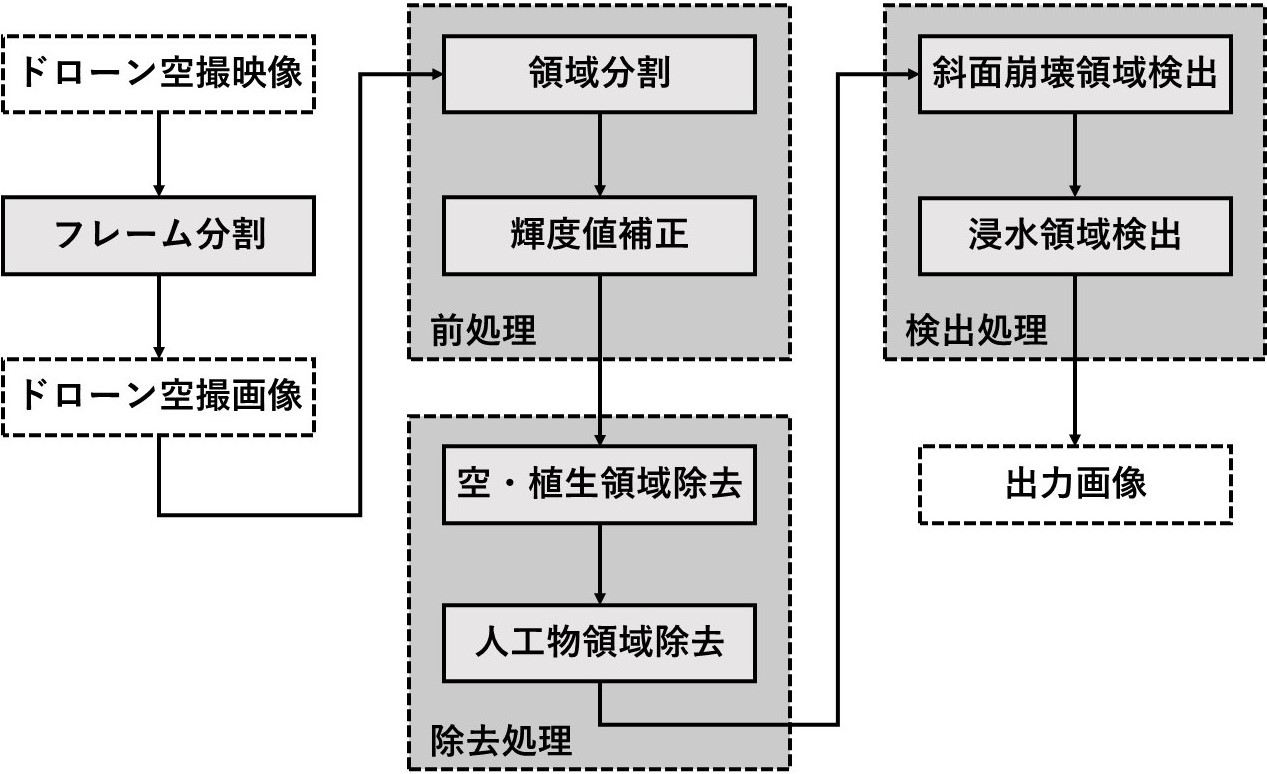
\includegraphics[width=8cm]{img/howto3.jpg}
% 	\caption{建物領域検出(実験Ⅱ)}
% 	\label{img18}
% \end{figure}

\subsection{統合処理}
	\ref{detection}にて検出した領域から\ref{rejection}にて検出した領域を除去し、最終出力結果とする。最終的に斜面崩壊と浸水領域を検出した結果を\fref{img19}~\fref{img20}に示す。


\begin{figure}[h]
	\centering
	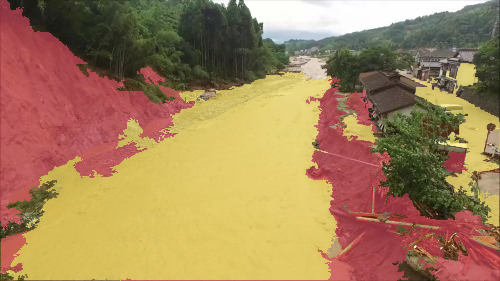
\includegraphics[width=8cm]{img/result1.png}
	\caption{最終出力結果(実験Ⅰ)}
	\label{img19}
\end{figure}
\begin{figure}[h]
	\centering
	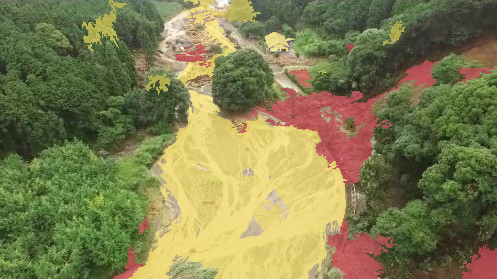
\includegraphics[width=8cm]{img/result2.png}
	\caption{最終出力結果(実験Ⅱ)}
	\label{img20}
\end{figure}


\section{精度評価}
目視判読による斜面崩壊・浸水領域の正解データを手動で作成し、画素数単位での適合率(precicsion)、再現率(recall)、F値(F-measure)にて精度評価を行った。適合率、再現率、F値の概念図と導出式を\fref{img21}とsiki{01}--siki{03}に示す。TP(True Positive)は正しく検出した画素、FP(False Positive)は誤検出した画素、FN(False Negative)は未検出の画素、TN(True Negative)は非検出対象画素を正しく未検出とした画素を表す。また、適合率は検出画素全体における正解画素の割合、再現率は正解画素全体における検出画素の割合、F値は適合率と再現率の調和平均で表した指標である。なお、F値の値が高い程精度が高いことを表す。最後に、本研究にて正解画像として作成した画像と精度評価結果を\fref{img22}と\fref{img23}、\tref{tab04}に示す。

\begin{figure}[h]
	\centering
	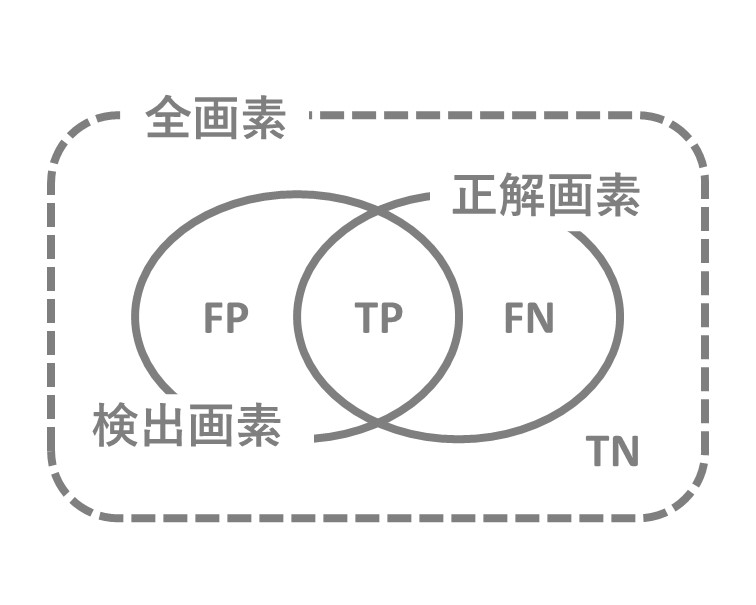
\includegraphics[width=8cm]{img/evaluation.jpg}
	\caption{精度評価概念図}
	\label{img21}
\end{figure}

\begin{equation}
	precicsion = \frac{TP}{TP+FP}
\end{equation}

\begin{equation}
	recall = \frac{TP}{TP+FN}
\end{equation}

\begin{equation}
	F_1 = \frac{2}{\frac{1}{recall}+\frac{1}{precicsion}} \\
	    = 2 \times \frac{recall*precicsion}{recall+precicsion}
\end{equation}

\begin{figure}[h]
	\centering
	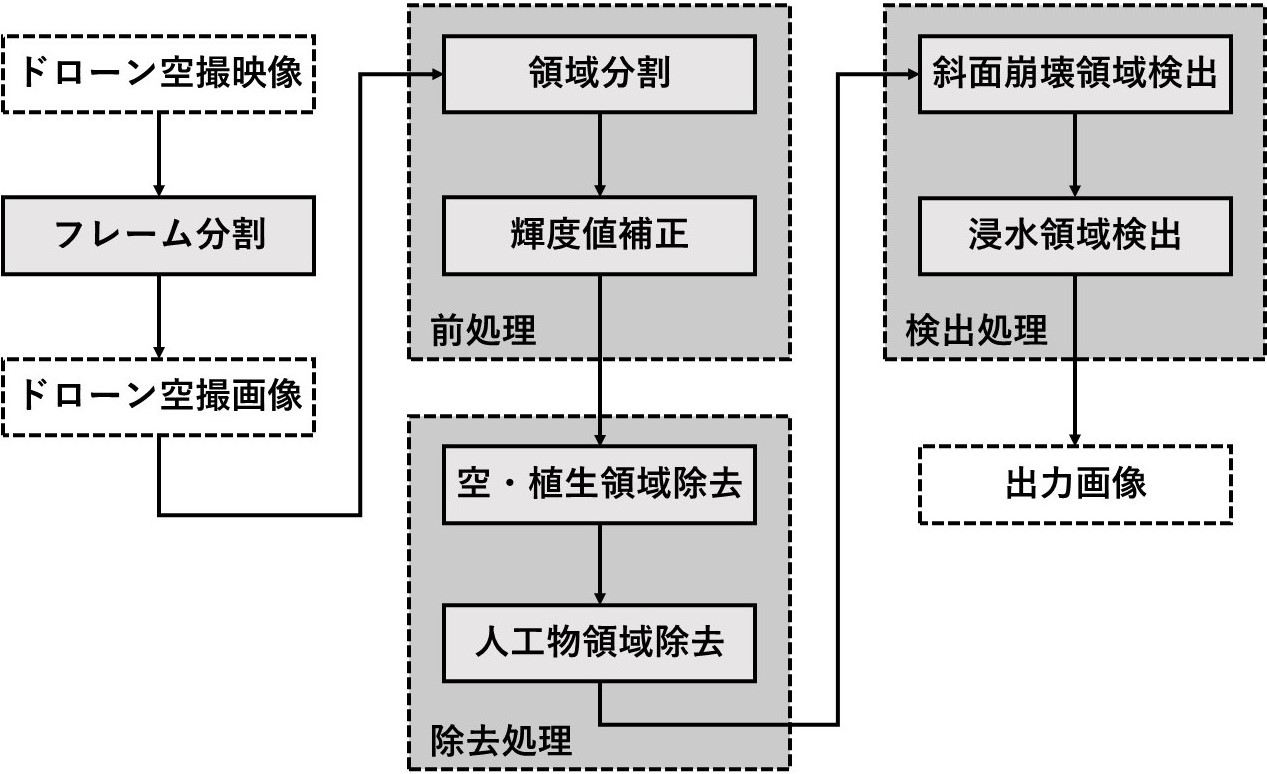
\includegraphics[width=8cm]{img/howto3.jpg}
	\caption{正解画像(実験Ⅰ)}
	% \caption{斜面崩壊領域正解画像(実験Ⅰ)}
	\label{img22}
\end{figure}
\begin{figure}[h]
	\centering
	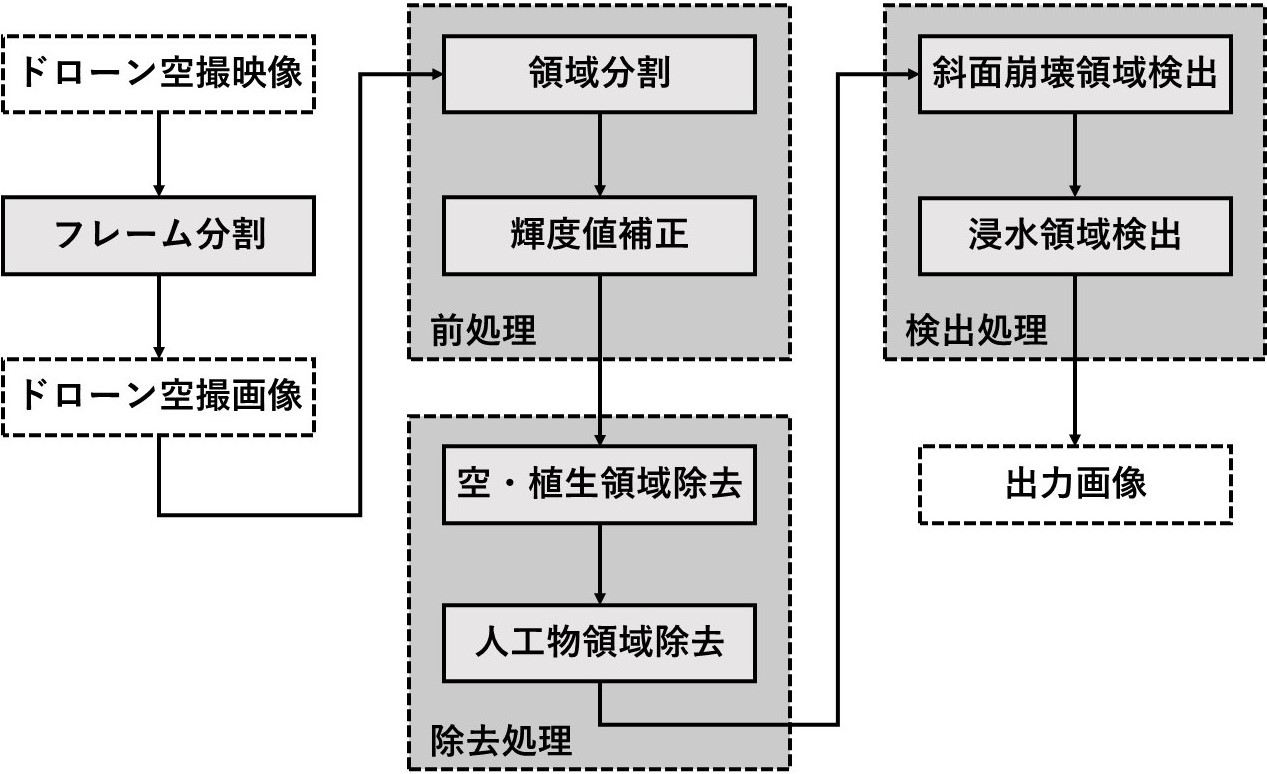
\includegraphics[width=8cm]{img/howto3.jpg}
	\caption{正解画像(実験Ⅱ)}
	% \caption{斜面崩壊領域正解画像(実験Ⅱ)}
	\label{img23}
\end{figure}

% \begin{figure}[h]
% 	\centering
% 	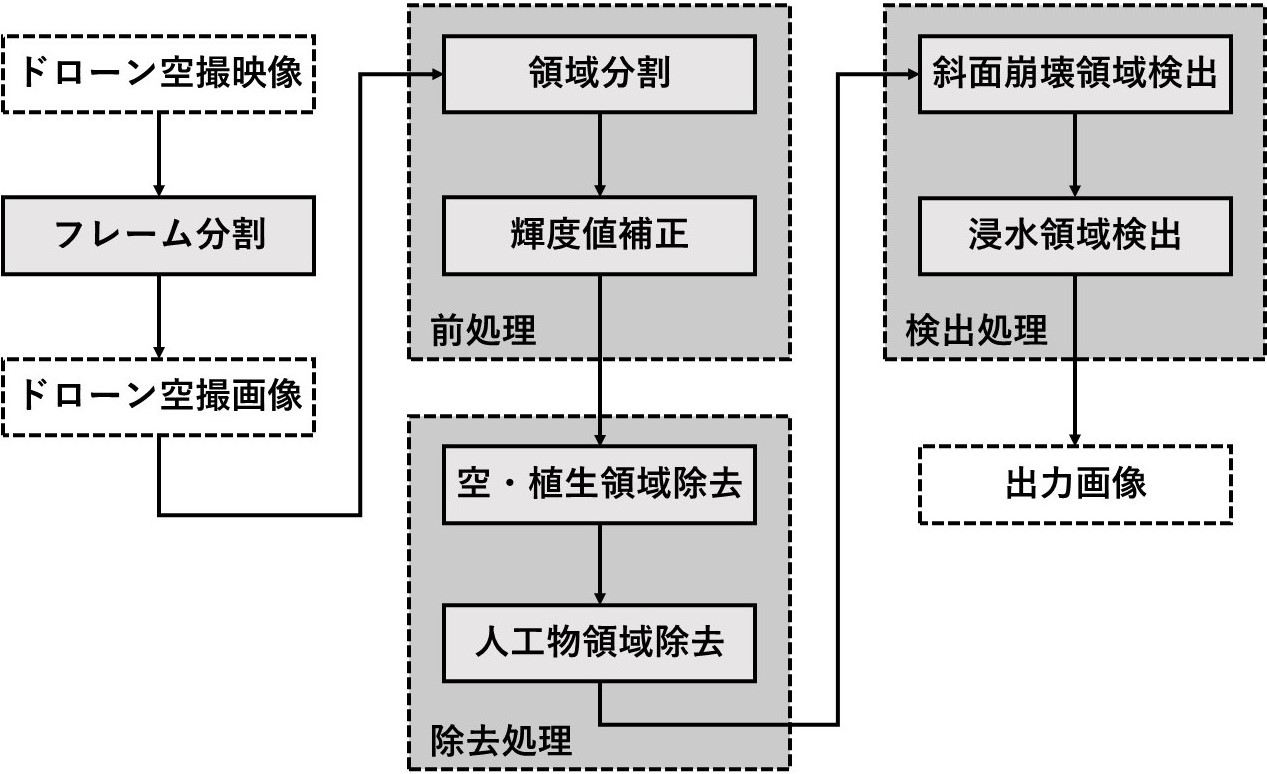
\includegraphics[width=8cm]{img/howto3.jpg}
% 	\caption{浸水領域正解画像(実験Ⅰ)}
% 	\label{img05}
% \end{figure}
% \begin{figure}[h]
% 	\centering
% 	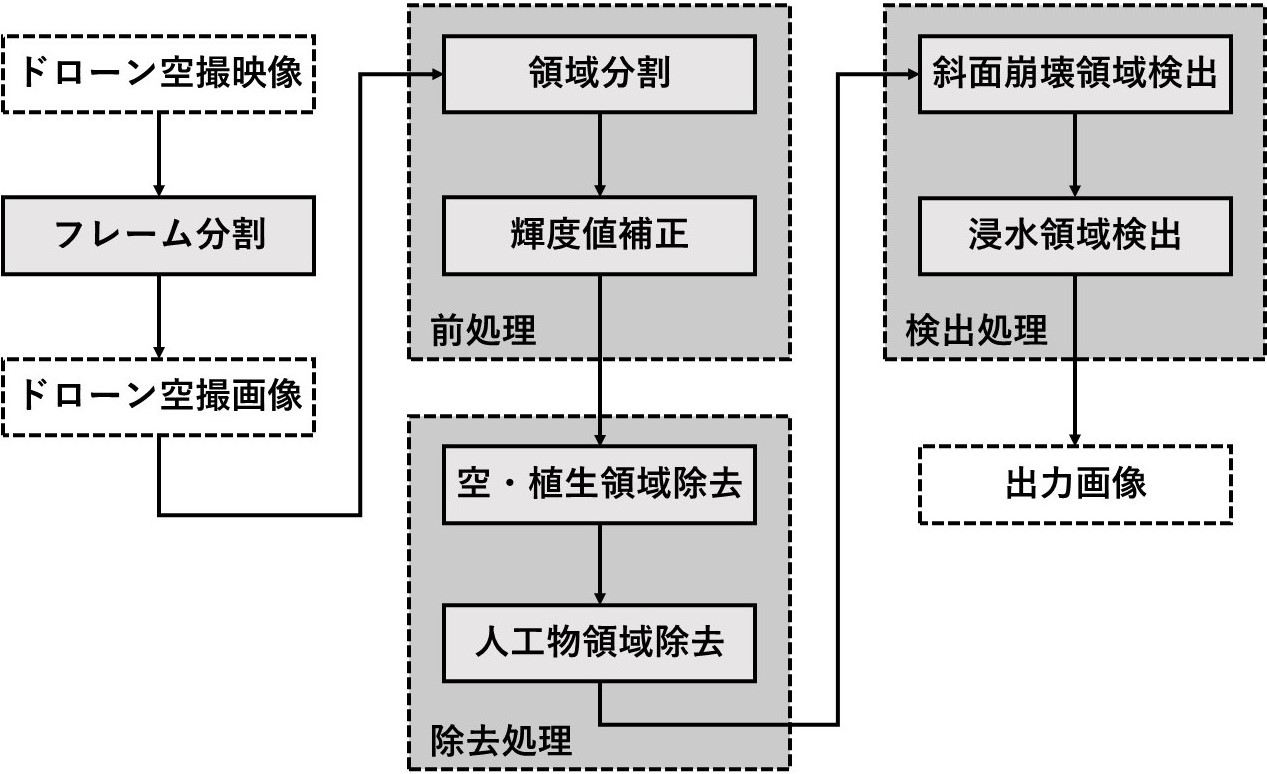
\includegraphics[width=8cm]{img/howto3.jpg}
% 	\caption{浸水領域正解画像(実験Ⅱ)}
% 	\label{img06}
% \end{figure}

\begin{table}[h]
	\centering
	\caption{精度評価}
	\label{tab04}
	\begin{tabular}{l l l l}
		\hline
		領域 & 適合率 & 再現率 & F値 \\
		斜面崩壊(実験Ⅰ) & 0.953 & 0.596 & 0.733 \\
		浸水(実験Ⅰ) & 0.848 & 0.987 & 0.912 \\
		斜面崩壊(実験Ⅱ) & 適合率 & 再現率 & F値 \\
		浸水(実験Ⅱ) & 適合率 & 再現率 & F値 \\
		\hline
	\end{tabular}
\end{table}


\section{考察}
	精度評価では~~~
	適合率、F値が以下の理由によってっっs
	推測すr



\end{document}
